\section{实验步骤}

本章节将展示实验步骤,包括生成复数型张量、傅立叶移位操作、傅立叶变换、傅立叶逆变换等。

\subsection{\texttt{commplex\_exp\_torch}函数的实现}

Pytorch中拥有不同的数据类型,包括整型、浮点型、复数型等。在Pytorch中,复数型数据类型为\texttt{torch.complex64}和\texttt{torch.complex128}。为了方便地生成复数型张量,本章节实现了\texttt{commplex\_exp\_torch}函数,用于生成复数型张量。

\begin{lstlisting}[style=Python]
def commplex_exp_torch(phase, dtype=torch.complex128):
    return torch.complex(torch.cos(phase), torch.sin(phase))
\end{lstlisting}

如上述代码所示,\texttt{commplex\_exp\_torch}函数接受一个\texttt{phase}参数,用于指定复数的相位。函数返回一个\texttt{torch.complex}类型的张量,其中实部为$\cos(\text{phase})$,虚部为$\sin(\text{phase})$。

\subsection{\texttt{fftshift2d\_tf}函数的实现}

傅立叶移位操作是指将频谱的零频率分量移动到频谱的中心位置。在Pytorch中,\texttt{torch.fft.fft2}函数返回的频谱是未移位的,即零频率分量位于频谱的左上角。为了方便地进行频谱的可视化,本章节实现了\texttt{fftshift2d\_tf}函数,用于对频谱进行移位操作。

\begin{lstlisting}[style=Python]
def ifftshift2d_tf(a_tensor):
    # (B, H, W, C)
    import math
    _, H, W, _ = a_tensor.size()
    H_split, W_split = math.ceil(H / 2), math.ceil(W / 2)
    a_tensor_up, a_tensor_down = a_tensor.split([H_split, H - H_split], dim=1)
    a_tensor = torch.cat([a_tensor_down, a_tensor_up], dim=1)
    a_tensor_left, a_tensor_right = a_tensor.split([W_split, W - W_split], dim=2)
    a_tensor = torch.cat([a_tensor_right, a_tensor_left], dim=2)
    return a_tensor
\end{lstlisting}

一维傅立叶移位操作是指将频谱的前一半数据移动到频谱的后一半位置。而二维如上述代码所示,\texttt{ifftshift2d\_tf}函数接受一个\texttt{a\_tensor}参数,用于指定需要移位的频谱。函数返回一个移位后的频谱。具体来说,函数首先将频谱沿着垂直方向分为上下两部分,然后将这两部分交换位置;接着将频谱沿着水平方向分为左右两部分,然后将这两部分交换位置。

% 子图1:tikz绘制2x2网格,左上、右上、左下、右下分别为1、2、3、4
% 子图2:上下翻转:3、4、1、2
% 子图3:左右翻转:4、3、2、1
% 采用subfloat排版
\begin{figure}[H]
    \centering
    \subfloat[原始频谱]{
        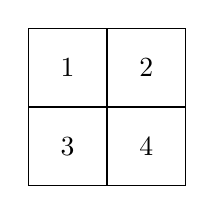
\begin{tikzpicture}
            \draw[step=1cm] (0,0) grid (2,2);
            \node at (0.5, 1.5) {1};
            \node at (1.5, 1.5) {2};
            \node at (0.5, 0.5) {3};
            \node at (1.5, 0.5) {4};
        \end{tikzpicture}
    }
    \subfloat[上下翻转]{
        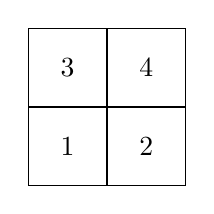
\begin{tikzpicture}
            \draw[step=1cm] (0,0) grid (2,2);
            \node at (0.5, 1.5) {3};
            \node at (1.5, 1.5) {4};
            \node at (0.5, 0.5) {1};
            \node at (1.5, 0.5) {2};
        \end{tikzpicture}
    }
    \subfloat[左右翻转]{
        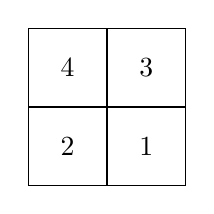
\begin{tikzpicture}
            \draw[step=1cm] (0,0) grid (2,2);
            \node at (0.5, 1.5) {4};
            \node at (1.5, 1.5) {3};
            \node at (0.5, 0.5) {2};
            \node at (1.5, 0.5) {1};
        \end{tikzpicture}
    }
    \caption{二维傅立叶移位操作}
\end{figure}

\subsection{\texttt{transp\_fft2d}函数的实现}

傅立叶变换是指将空间域信号转换为频谱。在Pytorch中,\texttt{torch.fft.fft2}函数用于计算二维傅立叶变换。为了方便地进行傅立叶变换操作,本章节实现了\texttt{transp\_fft2d}函数。

\begin{lstlisting}[style=Python]
def transp_fft2d(a_tensor, dtype=torch.complex64):
    # (B, H, W, C)
    return torch.fft.fft2(a_tensor, dim=(1, 2))
\end{lstlisting}

如上述代码所示,\texttt{transp\_fft2d}函数接受一个\texttt{a\_tensor}参数,用于指定需要进行傅立叶变换的信号。该函数对信号的高度、宽度维度进行傅立叶变换操作,返回一个复数类型的张量。

\subsection{\texttt{transp\_ifft2d}函数的实现}

傅立叶逆变换是指将频谱转换为空间域信号。在Pytorch中,\texttt{torch.fft.ifft2}函数用于计算二维傅立叶逆变换。为了方便地进行傅立叶逆变换操作,本章节实现了\texttt{transp\_ifft2d}函数。

\begin{lstlisting}[style=Python]
def transp_ifft2d(a_tensor, dtype=torch.complex64):
    # (B, H, W, C)
    return torch.fft.ifft2(a_tensor, dim=(1, 2))
\end{lstlisting}

如上述代码所示,\texttt{transp\_ifft2d}函数接受一个\texttt{a\_tensor}参数,用于指定需要进行傅立叶逆变换的频谱。该函数对频谱的高度、宽度维度进行傅立叶逆变换操作,返回一个复数类型的张量。

\subsection{运行脚本}

在编写完函数之后,可以在\texttt{proj5.ipynb}中进行测试。首先在目录下运行如下命令启动Jupyter Notebook:

\begin{lstlisting}[style=Bash]
jupyter notebook
\end{lstlisting}

之后在浏览器中打开\texttt{http://localhost:8888},点击\texttt{proj5.ipynb}文件,点击\texttt{Kernel}菜单下的\texttt{Restart \& Run All},即可运行整个脚本,如图\ref{fig:jupyter}所示。该脚本执行了模型训练和测试过程,与电子神经网络类似,模型通过\texttt{SGD}优化,损失函数为交叉熵损失函数,并采用\texttt{ReduceLROnPlateau}作为学习率调整策略,具体来说,当测试准确率连续2个epoch不再上升时,学习率将减小为原先的0.5倍。

\begin{figure}[H]
    \centering
    \includegraphics[width=0.8\textwidth]{pics/jupyter.png}
    \caption{Jupyter Notebook界面}
    \label{fig:jupyter}
\end{figure}
